\chapter{Estudio teórico. Propuestas en Positional Encoding}

En el capítulo anterior, presentamos los principales modelos de aprendizaje para series temporales, y así analizar las soluciones propuestas por cada uno. Al hacerlo, pudimos identificar un problema clave: la codificación posicional no recibe la atención necesaria, y en la mayoría de casos se usa la formulación original, con adaptaciones mínimas, o bien, es suprimido a favor de otras alternativas incorporadas en la propia arquitectura.\\

En este capítulo, teniendo presente los tipos anteriormente descritos de codificaciones (fijo, aprendible, adición de variables temporales, transformaciones), retomaremos esa clasificación para profundizar en las propuestas más recientes orientadas específicamente a series temporales, analizando su motivación, diseño y posibles ventajas frente a las formulaciones clásicas.\\

Partiremos del esquema tradicional de codificación posicional heredado del Transformer original y examinaremos cómo distintos trabajos recientes han intentado superar sus limitaciones mediante adaptaciones de carácter local o dependientes del contenido. Nuestro objetivo será identificar las ventajas concretas que aporta cada enfoque, extraer de ellos la inspiración necesaria y, a partir de ahí, diseñar nuevos experimentos de codificación posicional que integren ideas capaces de mejorar el rendimiento del modelo.

\section{Análisis de propuestas existentes}

Durante el análisis de los modelos más destacados del estado del arte, hemos podido ver en uso, principalmente, el mecanismo tradicional de atención basado en senos y cosenos, así como el basado en las transformadas de Fourier y Wavelet, en el caso de FEDformer. Sin embargo, dejando al margen estos enfoques, no hemos apreciado ninguna otra alternativa intuitiva que trate de mejorar el positional encoding más allá, ya que en otros casos, directamente se opta por su supresión o compensación por otro mecanismo.\\

Para poder profundizar más en este aspecto, podemos adentrarnos en surveys como el publicado por \textit{Habib Irani y Vangelis Metsis}~\cite{irani2025positionalencodingtransformerbasedtime}, donde se recogen multitud de variantes de encoding, aplicados a series temporales. Tomando como referencia la clasificación propuesta (ver figura \ref{encodings}), a continuación agruparemos las codificaciones posicionales en dos grandes categorías. Por un lado, aquellas que se incorporan sumándose directamente al embedding de entrada, conocidas como métodos absolutos de codificación posicional (APE); por otro, las que actúan modificando el propio cálculo de la atención, y que por ello se denominan métodos relativos de codificación posicional (RPE).


\begin{figure}[!ht]
	\centering
	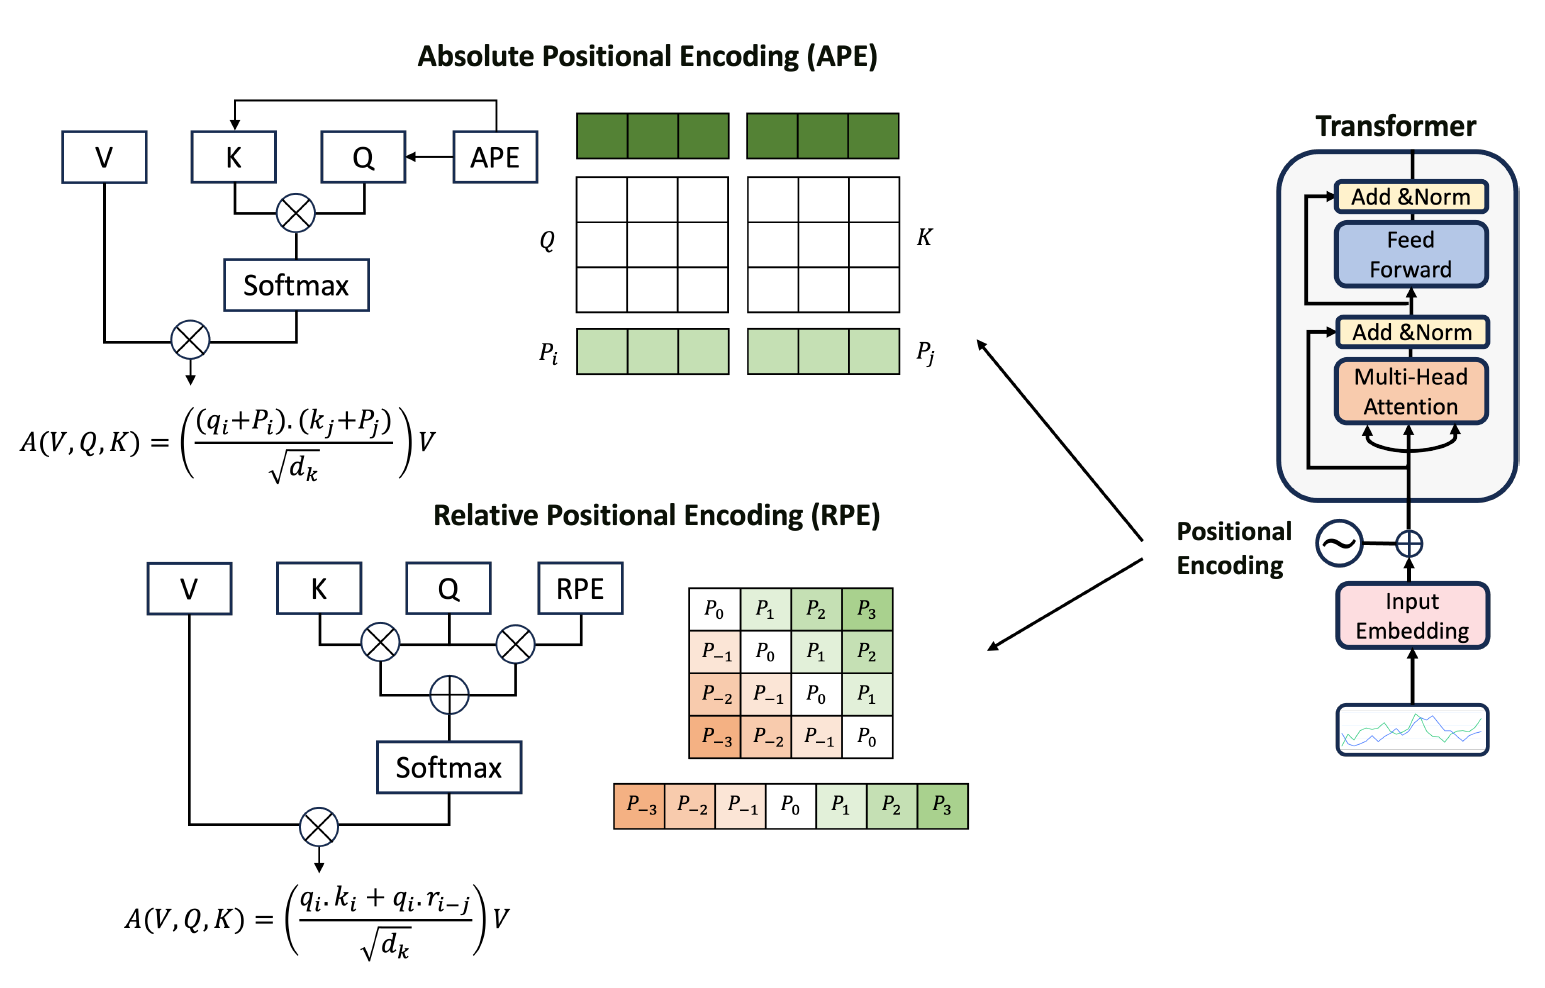
\includegraphics[scale=0.275]{img/encodings.png}
	\caption{Encodings: clasificación de métodos y funcionamiento \cite{irani2025positionalencodingtransformerbasedtime}}
	\label{encodings}
\end{figure}

\subsection{Métodos aditivos}

Comenzaremos el análisis por el positional encoding aditivo. Esta vertiente toma como referencia el mecanismo de adición de información empleado por el enfoque sinusoidal original, ya que todas estas codificaciones se añaden al embedding mediante suma, de forma que no es necesario realizar modificaciones adicionales a la arquitectura neural que los procesará, y facilita el uso de modelos preentrenados con el fin de ahorrar recursos de cómputo.\\

En mayor detalle, estos métodos construyen un vector posicional $(P \in \mathbb{R}^{L \times d})$ y lo se suma directamente a los embeddings de entrada (X), obteniendo:

$$ X' = X + P $$

donde (L) es la longitud de la secuencia y (d) la dimensión del embedding.\\

Suponen una ventaja desde el punto de vista de la usabilidad, ya que modificar excesivamente los mecanismos de atención puede dificultar su comprensión y provocar efectos adversos indeseados si no se realiza con el rigor necesario. A continuación, destacaremos algunos de los mecanismos existentes con estas características, y analizaremos la utilidad ofrecida por cada uno.

\subsubsection{Sinusoidal Positional Encoding (PE)}

Se trata del encoding original propuesto originalmente por Vaswani et al. (2017)~\cite{vaswani2023attentionneed}, a modo de recordatorio. Como ya vimos, utiliza funciones sinusoidales para representar la posición:

$$
PE_{(pos, 2i)} = \sin\left(\frac{pos}{10000^{\frac{2i}{d}}}\right)
$$

$$
PE_{(pos, 2i+1)} = \cos\left(\frac{pos}{10000^{\frac{2i}{d}}}\right)
$$

Donde cada variable indica:

\begin{itemize}
	\item \textbf{pos}: índice temporal (posición).
	\item \textbf{i}: dimensión del componente del embedding.
	\item \textbf{d}: dimensión total del embedding.
\end{itemize}

Basándonos simplemente en su formulación, fuimos capaces de distinguir ya sus ventajas y desventajas; como ventaja, podemos ver que se trata de una codificación no entrenable, por lo que para unas mismas dimensiones de entrada de datos, el resultado será siempre el mismo, y sus valores no se deben entrenar época a época de manera independiente. Esto lo hace más sencillo de usar, y más eficiente al no requerir parámetros adicionales. Sin embargo, como principal desventaja, estimamos que no permite modelar con suficiente adaptabilidad los períodos no estacionales de datos o con mayor número de irregularidades y valores anómalos.\\

Su forma sencilla de acoplar al conjunto de datos de entrada nos sirve de inspiración para la creación de nuevas variantes que traten de incorporar más contexto semántico de los datos.

\subsubsection{Time Absolute Positional Encoding (tAPE)}

tAPE propone una solución que, aunque sigue perteneciendo a la familia de codificaciones fijas, incorpora información estructural propia de la secuencia de entrada, en particular su longitud real $L$. La idea central es ajustar la escala de las frecuencias empleadas en la codificación sinusoidal en función de esa longitud, de forma que la representación posicional conserve una propiedad conocida como \textit{distance-awareness}.\\

Por \textit{distance-awareness} entendemos la capacidad de la codificación para reflejar, de manera coherente y diferenciada, la distancia relativa entre posiciones, y así complementar a la información global. En una codificación con buena distance-awareness, dos posiciones cercanas deben tener representaciones más similares entre sí que respecto a posiciones muy alejadas, y esta relación se mantiene de forma proporcional a lo largo de toda la secuencia. Es algo que no logramos cosneguir en codificaciones sinusoidales estándar, sobre todo cuando la dimensión del embedding es baja, ya que las frecuencias asignadas no siempre proporcionan suficiente resolución para representar distancias cortas.\\

Para mitigar este problema, tAPE redefine las frecuencias como:

\begin{equation}
	\centering
	\omega^{new}_k = k \cdot \frac{d_{model}}{L}
\end{equation}

Adaptando así su espectro al tamaño real de la secuencia y adecuándose incluso a casos de entrada de corta longitud. Esta nueva frecuencia simplemente se incorpora como parámetro a la codificación sinusoidal estándar:

\begin{equation}
	\begin{aligned}
		\text{PE}_{(pos,2i)} &= \sin\!\left( pos \cdot \omega^{new}_i \right) \\
		\text{PE}_{(pos,2i+1)} &= \cos\!\left( pos \cdot \omega^{new}_i \right)
	\end{aligned}
\end{equation}


Donde:

\begin{itemize}
	\item \textit{d} representa la dimensión del embedding utilizada por el modelo Transformer; este valor determina el número de componentes de la codificación posicional y, por tanto, el rango de frecuencias disponibles para representar las posiciones.
	\item \textit{L} corresponde a la longitud real de la secuencia.
	\item \textit{k} es el índice de la dimensión o de la frecuencia dentro del embedding; al recorrer k desde valores bajos a altos, obtenemos frecuencias cada vez más elevadas en las funciones seno y coseno, lo que permite representar tanto variaciones lentas (baja frecuencia) como rápidas (alta frecuencia) a lo largo de la secuencia.
\end{itemize} 

La principal virtud de tAPE es su capacidad para mantener la distance-awareness incluso en contextos con embeddings de baja dimensión, algo que no siempre se logra con la codificación sinusoidal estándar. Al incorporar la longitud real \textit{L} en el cálculo de las frecuencias, se evita que la escala sea excesivamente grande o pequeña para la secuencia procesada, lo que redunda en una representación posicional más ajustada y fiel a las distancias relativas. Esta adaptación es especialmente útil en series temporales de corta o media duración, donde las relaciones locales y su correcta discriminación son fundamentales.\\

Sin embargo, sigue teniendo limitaciones evidentes. Para empezar, su dependencia explícita de \textit{L} puede suponer un problema si, durante la inferencia, trabajamos con secuencias de longitud muy distinta a la usada en el entrenamiento, aunque normalmente, se deberían seguir distribuciones similares. Además, tAPE es un método de codificación fijo y no incorpora parámetros aprendibles, lo que si bien simplifica su uso y evita sobreajuste, también le impide adaptarse dinámicamente a patrones posicionales más complejos o irregulares presentes en diferentes dominios o conjuntos de datos.

\subsubsection{Learnable Positional Encoding (LPE)}

En el método sinusoidal tradicional, la codificación posicional se realizaba de forma fija e invariante, dependiendo únicamente de las dimensiones de los datos de entrada. Sin embargo, esto no favorece a la localización de estructuras y detalles propios de los datos de entrada, por lo que surge así el encoding posicional aprendible. Su filosofía se basa en dejar que el modelo sea quien entrene los valores de la codificación posicional a la vez que el resto de la arquitectura se refina:

$$
PE_{\text{learnable}}(pos) = W_{pos}, \quad W_{pos} \in \mathbb{R}^d
$$

Esta codificación aprendida se incorpora al embedding de entrada de manera aditiva como hasta ahora:


$$
X' = X + PE_{\text{learnable}}[pos]
$$

La principal fortaleza de este método reside en su capacidad de adaptación. A diferencia de métodos como el PE sinusoidal o tAPE, que imponen un patrón posicional fijo, LPE permite que el modelo aprenda directamente, a partir de los datos, la representación posicional que mejor captura las relaciones temporales y estructurales relevantes para la tarea. Esta flexibilidad puede traducirse en una mayor precisión, especialmente en dominios donde las dependencias posicionales no siguen un patrón excesivamente regular, o cuando la información contextual es altamente específica del conjunto de datos y es compleja de detectar de manera intuitiva.\\

No obstante, esta flexibilidad tiene un precio. Al añadir un vector de parámetros por cada posición, el tamaño del modelo crece linealmente dependiendo del parámetro de longitud \textit{L}, lo que incrementa tanto el coste de almacenamiento como el de entrenamiento. Además, la codificación aprendida queda estrechamente ligada al conjunto de datos utilizado para ajustarla; esto implica que, ante un cambio de dominio o de distribución de las secuencias, incluso si la longitud se mantiene, es necesario volver a entrenar los embeddings posicionales desde cero para preservar su utilidad. En contraste con tAPE, que conserva su aplicabilidad en distintos contextos gracias a su formulación fija, LPE sacrifica generalidad en favor de especialización.


\subsubsection{Temporal Positional Encoding (T-PE)}

Por último, nos centraremos en el encoding posicional temporal (T-PE), un enfoque híbrido que combina información posicional global y dependiente del contenido para enriquecer la representación. Por un lado, emplea la codificación geométrica sinusoidal clásica para la parte absoluta, para dotar al modelo de información posicional estable y determinista. Por otro lado, T-PE integra una componente semántica basada en similitud entre embeddings de los datos, que añade un sesgo contextual para capturar relaciones entre posiciones no solo por su índice temporal, sino también por su contenido o características. Esto se consigue mediante una función de suavizado gaussiano que mide la proximidad en el espacio de características entre cada par de posiciones. De esta forma, aportamos la visión semántica, elemento que principalmente queda infrarrepresentado en modelos fijos.\\

Formalmente, el modelo basa su componente geométrica mediante:

\begin{equation}
	PE_{i, 2k} = \sin\left(\frac{i}{10000^{\frac{2k}{d}}}\right), \quad
	PE_{i, 2k+1} = \cos\left(\frac{i}{10000^{\frac{2k}{d}}}\right)
\end{equation}

Y la componente semántica, que mide la similitud local entre embeddings, se define como:

$$S(i, j) = \exp\left( -\frac{\|x_i - x_j\|^2}{2\sigma^2} \right)$$

Añadiéndose al encoding final de manera aditiva:

$$T\text{-}PE(i) = PE(i) + S(i, j)$$


La principal fortaleza de este enfoque, por tanto, radica en la combinación de un anclaje posicional absoluto con una componente semántica adaptativa, lo que le permite capturar, de forma natural y simultánea, tanto las relaciones temporales globales como las similitudes entre elementos, integrando información global y local en una única representación.\\

Pero su implementación puede inducir problemas para la escalabilidad. La gaussiana entre todas las posiciones implica un coste cuadrático $O(L^2)$.- Además, su rendimiento está fuertemente condicionado por el grado de integración entre las dos componentes, ya que un desbalance podría anular las ventajas buscadas.\\

En resumen, T-PE propone un enfoque híbrido bastante interesante, capaz de emplear las ventajas del contenido estructural y el semántico.


\subsection{Métodos que manipulan la atención}

Hasta ahora, hemos explorado tres métodos de codificación posicional que comparten un rasgo común: todos operan mediante una simple suma dentro del embedding de entrada. Sin embargo, existe otra vía para mejorar el desempeño de los modelos Transformer que va más allá de la manipulación directa del embedding: intervenir directamente en el mecanismo de atención.\\

Hasta el momento, las modificaciones de atención que hemos visto se basaban principalmente en técnicas de muestreo para reducir el tamaño del producto, seleccionando un subconjunto de productos en lugar de trabajar con la matriz completa. Aunque estas estrategias mejoran la eficiencia, en esencia mantienen el mismo trasfondo matemático. Para avanzar más allá, podemos especializar el cálculo de la atención para que incorpore de manera explícita la estructura propia de las series temporales. De este modo, es en el propio proceso de atención, y durante la fase de creación del embedding, donde el modelo puede captar de manera más efectiva las dependencias temporales y las características relevantes del dominio, potenciando así su capacidad de predicción a largo plazo. A continuación, examinaremos algunos de los métodos propuestos y su funcionamiento

\subsubsection{Relative Positional Encoding (RPE)}


Una de las principales limitaciones del encoding posicional absoluto es que se basa en posiciones fijas e independientes, sin considerar cómo se relacionan entre sí los elementos en la secuencia. Mediante esta propuesta, el RPE, mejoramos el mecanismo de atención incorporando explícitamente un término que depende de la \emph{posición relativa} entre elementos, en lugar de usar solo sus posiciones absolutas.\\

Esta característica permite que el modelo capture relaciones y patrones que se mantienen constantes sin importar el punto exacto en la secuencia donde ocurren, haciendo que la atención sea más flexible y adaptativa. Desde un punto de vista matemático, la energía de atención entre los elementos en las posiciones \(i\) y \(j\) se calcula como:


\[
e_{ij} = \frac{(x_i W_Q)(x_j W_K)^\top}{\sqrt{d_z}} + \frac{(x_i W_Q)(a^K_{ij})^\top}{\sqrt{d_z}}, \quad \text{donde} \quad a^K_{ij} = W^r_K r_{i-j}
\]

Aquí, \(r_{i-j}\) representa un embedding que codifica la distancia relativa entre las posiciones \(i\) y \(j\). Las matrices \(W_Q\) y \(W_K\) son las matrices de proyección aprendibles para las queries y las keys, respectivamente, mientras que \(W^r_K\) es la proyección asociada a los embeddings relativos. El término \(d_z\) corresponde a la dimensión de las representaciones en la atención.\\

Este enfoque permite capturar relaciones relativas invariantes a traslaciones en la secuencia, lo cual resulta especialmente beneficioso para tareas en las que la distancia entre elementos es más importante que su posición absoluta. Por ello, mejora la capacidad de generalización del modelo frente a variaciones en la posición, y es especialmente útil en problemas de predicción, o clasificación, que poseen longitudes de secuencia variables.\\

Sin embargo, esta mejora tiene un coste: se incrementa tanto la complejidad computacional como el consumo de memoria, manteniéndose en orden \(O(L^2)\). Además, la implementación requiere almacenar y gestionar tablas de embeddings relativos para todas las posibles distancias, lo que puede complicar enormemente su escalabilidad en secuencias de larga duración.


\subsubsection{Efficient Relative Positional Encoding (eRPE)}

El modelo RPE anteriormente muestra una gran utilidad en series cambiantes, pero su eficiencia computacional costosa podría ser una gran limitación de uso. Por ello, existe una variante llamada eRPE, donde el sesgo relativo de las posiciones se incorpora después de aplicar la función Softmax en el cálculo de la atención. Es decir, en lugar de modificar la energía de atención antes de la normalización, el ajuste relativo se añade directamente sobre la distribución de atención ya calculada.

Formalmente, la atención sobre el elemento en la posición \(i\) se define como:

\[
\alpha_i = \sum_{j \in L} \left( \frac{\exp(e_{i,j})}{\sum_{k \in L} \exp(e_{i,k})} Ai,j + w_{i-j} \right) x_j
\]

donde \(w_{i-j}\) es un vector aprendible de  tamaño $2L - 1$. Dicho elemento es agregado tras realizar el proceso de atención, fuera de la Softmax. Así, la atención puede ajustarse localmente para enfatizar o atenuar ciertas posiciones relativas sin distorsionar la distribución global.\\

 Si bien dicha delimitación de tamaño de \textit{w} puede mejorar considerablemente el uso de memoria, acentúa la importancia de la información poisicional del embedding, por lo que se especializa su uso principalmente para tareas de clasificación, que se desvía de nuestro actual propósito de forecasting.

\subsubsection{Transformer with Untied Positional Encoding (TUPE)}

El modelo TUPE propone una formulación diferente a la vista hasta el momento con RPE: separa explícitamente la información de contenido y la información posicional durante el cálculo de la atención, evitando que ambas se mezclen o interfieran entre sí.\\

Matemáticamente, la atención entre los elementos en las posiciones \(i\) y \(j\) se calcula como la suma de dos términos:

\begin{equation}
	\alpha_{ij} = \frac{1}{\sqrt{2d}} (x_i^l W^{Q,l})\cdot(x_j^l W^{K,l})^T + \mathrm{reset}_\theta(\beta_{ij}, i, j)
\end{equation}

\begin{equation}
	\beta_{ij} = \frac{1}{\sqrt{2d}} (p_i U_Q)(p_j U_K)^T
\end{equation}

Donde $\beta_{ij}$ representa las interacciones entre posiciones; \(x_i\) representa el embedding de contenido en la posición \(i\), mientras que \(p_i\) es el embedding posicional correspondiente.\\

Esta separación evita la interferencia entre los patrones de contenido y los posicionales, permitiendo que cada componente se aprenda de forma independiente. Para datos de series temporales, esto resulta especialmente útil, ya que permite al modelo capturar tanto los patrones temporales (a través de las correlaciones posicionales) como las relaciones entre características (a través de las correlaciones de contenido) sin que ambos se interfieran mutuamente.\\

Debemos tener especial cuidado al usar este método en conjuntos de datos pequeños, ya que su mayor cantidad de parámetros puede suponer fácilmente problemas de sobreaprendizaje, los cuales tendremos que gestionar.


\subsubsection{Convolutional Stochastic Positional Encoding (Conv-SPE)}

Para cerrar el grupo de métodos que modifican la atención, tenemos Conv-SPE. Como indica su nombre, en lugar de usar codificaciones fijas o vectores aprendibles asociados a posiciones, utiliza convoluciones para capturar patrones locales y dependencias espaciales en la codificación posicional. Este enfoque se proponer a priori por ser más flexible y adaptativo, permitiendo modelar relaciones complejas a distintas escalas, incorporando un sesgo inductivo beneficioso para series temporales y mejorando la eficiencia y robustez en la captura de dependencias posicionales. \\

Su formulación comienza generando una matriz aleatoria \( Z_d \in \mathbb{R}^{M \times R} \) cuyos elementos siguen una distribución gaussiana estándar independiente e idénticamente distribuida (i.i.d.). Sobre esta matriz, se aplican filtros convolucionales aprendibles \(\Phi^Q\) y \(\Phi^K\) para transformar la información posicional en representaciones útiles para la atención:

\begin{equation}
Q_d = Z_d \otimes \Phi^Q, \quad K_d = Z_d \otimes \Phi^K
\end{equation}

Aquí, \(\otimes\) denota la operación de convolución, que consiste en aplicar un filtro móvil que recorre la matriz \(Z_d\) para extraer características locales, y \(\Phi^Q, \Phi^K\) son esos filtros que el modelo aprende durante el entrenamiento.\\

La clave de este método es que la operación de convolución, al ser local por naturaleza, captura patrones y relaciones cercanas dentro de los datos, otorgando así una estructura inductiva que se adapta a las dependencias temporales y espaciales presentes en las series temporales.\\

Además, cuando el parámetro \(R\) es suficientemente grande, la matriz resultante de estas convoluciones tiene una estructura de varianza cruzada que se aproxima al kernel de atención tradicional. Esto permite que la atención se pueda estimar de manera eficiente mediante el producto:

\begin{equation}
	P_d \approx \frac{\bar{Q}_d \bar{K}_d^T}{R}
\end{equation}

donde \(\bar{Q}_d\) y \(\bar{K}_d\) son las representaciones convolucionales normalizadas.\\

Sobre el papel, presenta varias ventajas. En primer lugar, captura relaciones relativas sin requerir atención cuadrática, gracias a la estimación realizada que es de orden lineal, facilitando su escalabilidad. Además, es más robusta ante sobreajuste por su componente estocástico. Sin embargo, aunque en principio pueda parecer más eficiente, modificar el mecanismo de atención puede ser delicado y su rendimiento depende mucho del conjunto de datos utilizado. De hecho, sus creadores señalan que este enfoque es más adecuado para tareas de clasificación de series temporales que para tareas de predicción, por lo que su aplicabilidad se aleja del contexto de este trabajo.

\section{Formulación de nuevas alternativas de PE}

Una vez analizadas todas las propuestas más destacadas a fecha de 2025 \cite{irani2025positionalencodingtransformerbasedtime}, es momento de formular nuestras propias alternativas que sean capaces de aprovechar los conceptos vistos hasta el momento, pero, aporten un nuevo enfoque que nos permita obtener buenos resultados. En este apartado, analizaremos los diferentes pilares que compondrán nuestras alternativas, que serán examinadas y evaluadas para verificar si cumplen con los estándares mínimos de rendimiento.

\subsection{Criterios de partida}

Para comenzar, estableceremos los criterios que vamos a seguir en la formulación de las alternativas, y la justificación de la toma de decisiones.\\

La primera cuestión que nos puede emerger es el tipo de encoding que parece más conveniente: un encoding aditivo, más sencillo e intuitivo de formular, o bien, un encoding basado en modificar el mecanismo de atención. Con la experiencia recogida de los ejemplos vistos en subapartado anterior, responder a esta pregunta es sencillo; los mecanismos de modificación de la atención parecen una mejora razonable sobre el papel, pero el overhead introducido sobre el tiempo de entrenamiento puede ser excesivo, ralentizando en exceso los experimentos dados los recursos disponibles para realizar este proyecto. Además, hemos podido verificar que prácticamente todos los métodos recogidos en el survey funcionan especialmente mejor para tareas de clasificación, lo cual es un problema totalmente diferente frente a nuestro propósito de realizar forecasting. En definitiva, si bien ejecutaremos alguna prueba puntual con este tipo de algoritmos para verificar su eficiencia y rendimiento, no será nuestro camino a seguir.\\

En su lugar, optaremos por modelos que modifiquen únicamente el embedding de entrada, pero no alteren la arquitectura del Transformer propiamente dicha, centrándonos en un objetivo clave: mejorar la semántica de los datos, empleando para ello la información local de los propios datos. A excepción de LPE y la parte semántica de T-PE, la mayoría de modelos de encoding son agnósticos al contenido del conjunto de entrenamiento, y debemos tratar de solucionar este problema. Para ello, podemos tomar inspiración de los primeros modelos de cálculo, como ARIMA y STL, y recuperar uno de los conceptos no empleados hasta ahora: el uso de ventanas. Pero no desde el punto de vista de troceado del conjunto de datos, sino como herramienta para construir localidad espacial.\\

Podemos lograr que entornos locales de similares características tengan una codificación también muy parecida, y la propia arquitectura del Transformer sea capaz de identificar dichas entradas similares para construir patrones de estacionalidad y puntos de interés. Para ello, un modelo aditivo puro podría dificultar la percepción de qué información es la de contexto de entrada, y cual es la información posicional. Por tanto, a diferencia de lo visto hasta ahora, podemos plantear una solución alternativa: concatenar esta información al embedding de entrada, aumentando su dimensionalidad en cuanto a número de características, pero facilitando dicha separación.\\

Como contenido a añadir, la idea más simple consiste en utilizar estadísticos básicos: medidas fácilmente paralelizables y sencillas en cómputo que, evaluadas entorno a una ventana para cada valor, nos pueda ofrecer nuevas características. Pueden ser desde métricas básicas de dispersión y valores extremos, hasta diferencias entre el valor central $x$ y el lag de orden n, $x_n$. De esta forma, potenciamos el modelado de la información alrededor de cada punto, y es potencialmente probable que dos valores $x$ separados en la serie, con un mismo contexto de valores locales concatenados, realmente se encuentren en las mismas posiciones relativas a un período de una estación.\\

Pero, esta idea no tiene por qué entrar en conflicto con el resto de codificaciones existentes; podemos beneficiarnos de un modelo de PE combinado entre el método de concatenación de valores provenientes de ventanas y las formas de codificación aditivas clásicas vistas ahora, de manera que nuestro método no se excluyen, y se beneficie de estas otras codificaciones. Esta idea ya se menciona en \cite{irani2025positionalencodingtransformerbasedtime} en relación a compatibilizar el uso de métodos aditivos y modificadores de atención (figura \ref{hybridpaper}), pero podemos adoptarlo para inspirarnos en un concepto similar: la combinación de método propuesto de concatenación, fruto de operaciones en la ventana, con un conjunto ponderado de PE aditivos de los ya vistos.\\

\begin{figure}[!ht]
	\centering
	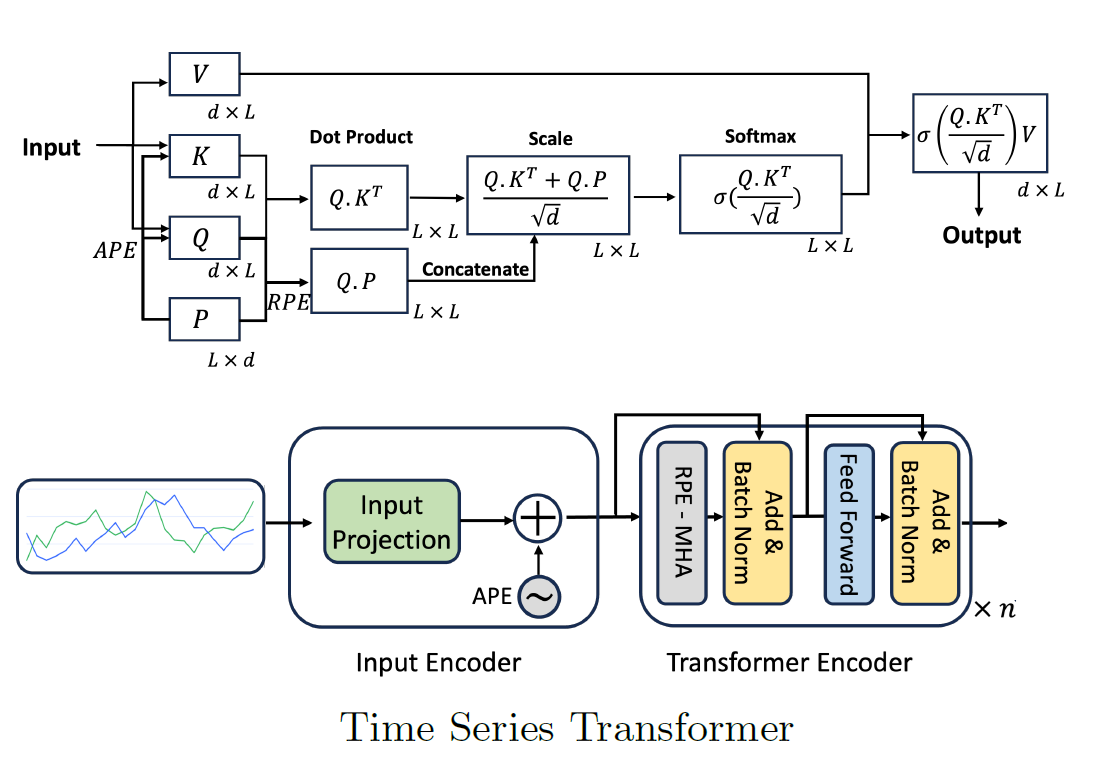
\includegraphics[scale=0.35]{img/hybridpaper.png}
	\caption{Codificación híbrida: métodos aditivos + atención \cite{irani2025positionalencodingtransformerbasedtime}}
	\label{hybridpaper}
\end{figure}


Proponemos así dotar a cada encoding aditivo de un peso aprendible para que el modelo seleccione automáticamente cuáles contribuyen más al embedding final. Si el peso de un encoding se aproxima a 0, ese encoding queda efectivamente suprimido de la ecuación, permitiendo que prevalezcan los métodos que realmente aportan información al embedding final. No obstante, esta propuesta requiere especial cuidado: sin restricciones, algunos pesos pueden crecer de forma desproporcionada (o bien desvanecerse), impidiendo la convergencia, y por tanto, la cercanía a soluciones óptimas. Una solución simple es aplicar un mecanismo de normalización de pesos, como forzar que los pesos sumen 1. Esto lo podemos conseguir de forma sencilla mediante Softmax, que actúa como regularizador y estabiliza la ponderación entre encodings. Adicionalmente, podría ser interesante combinarlo con inicializaciones acotadas, con valores pequeños. Su definición puede apeciarse gráficamente en la figura \ref{enhancedhybrid}.\\

\begin{figure}[!ht]
	\centering
	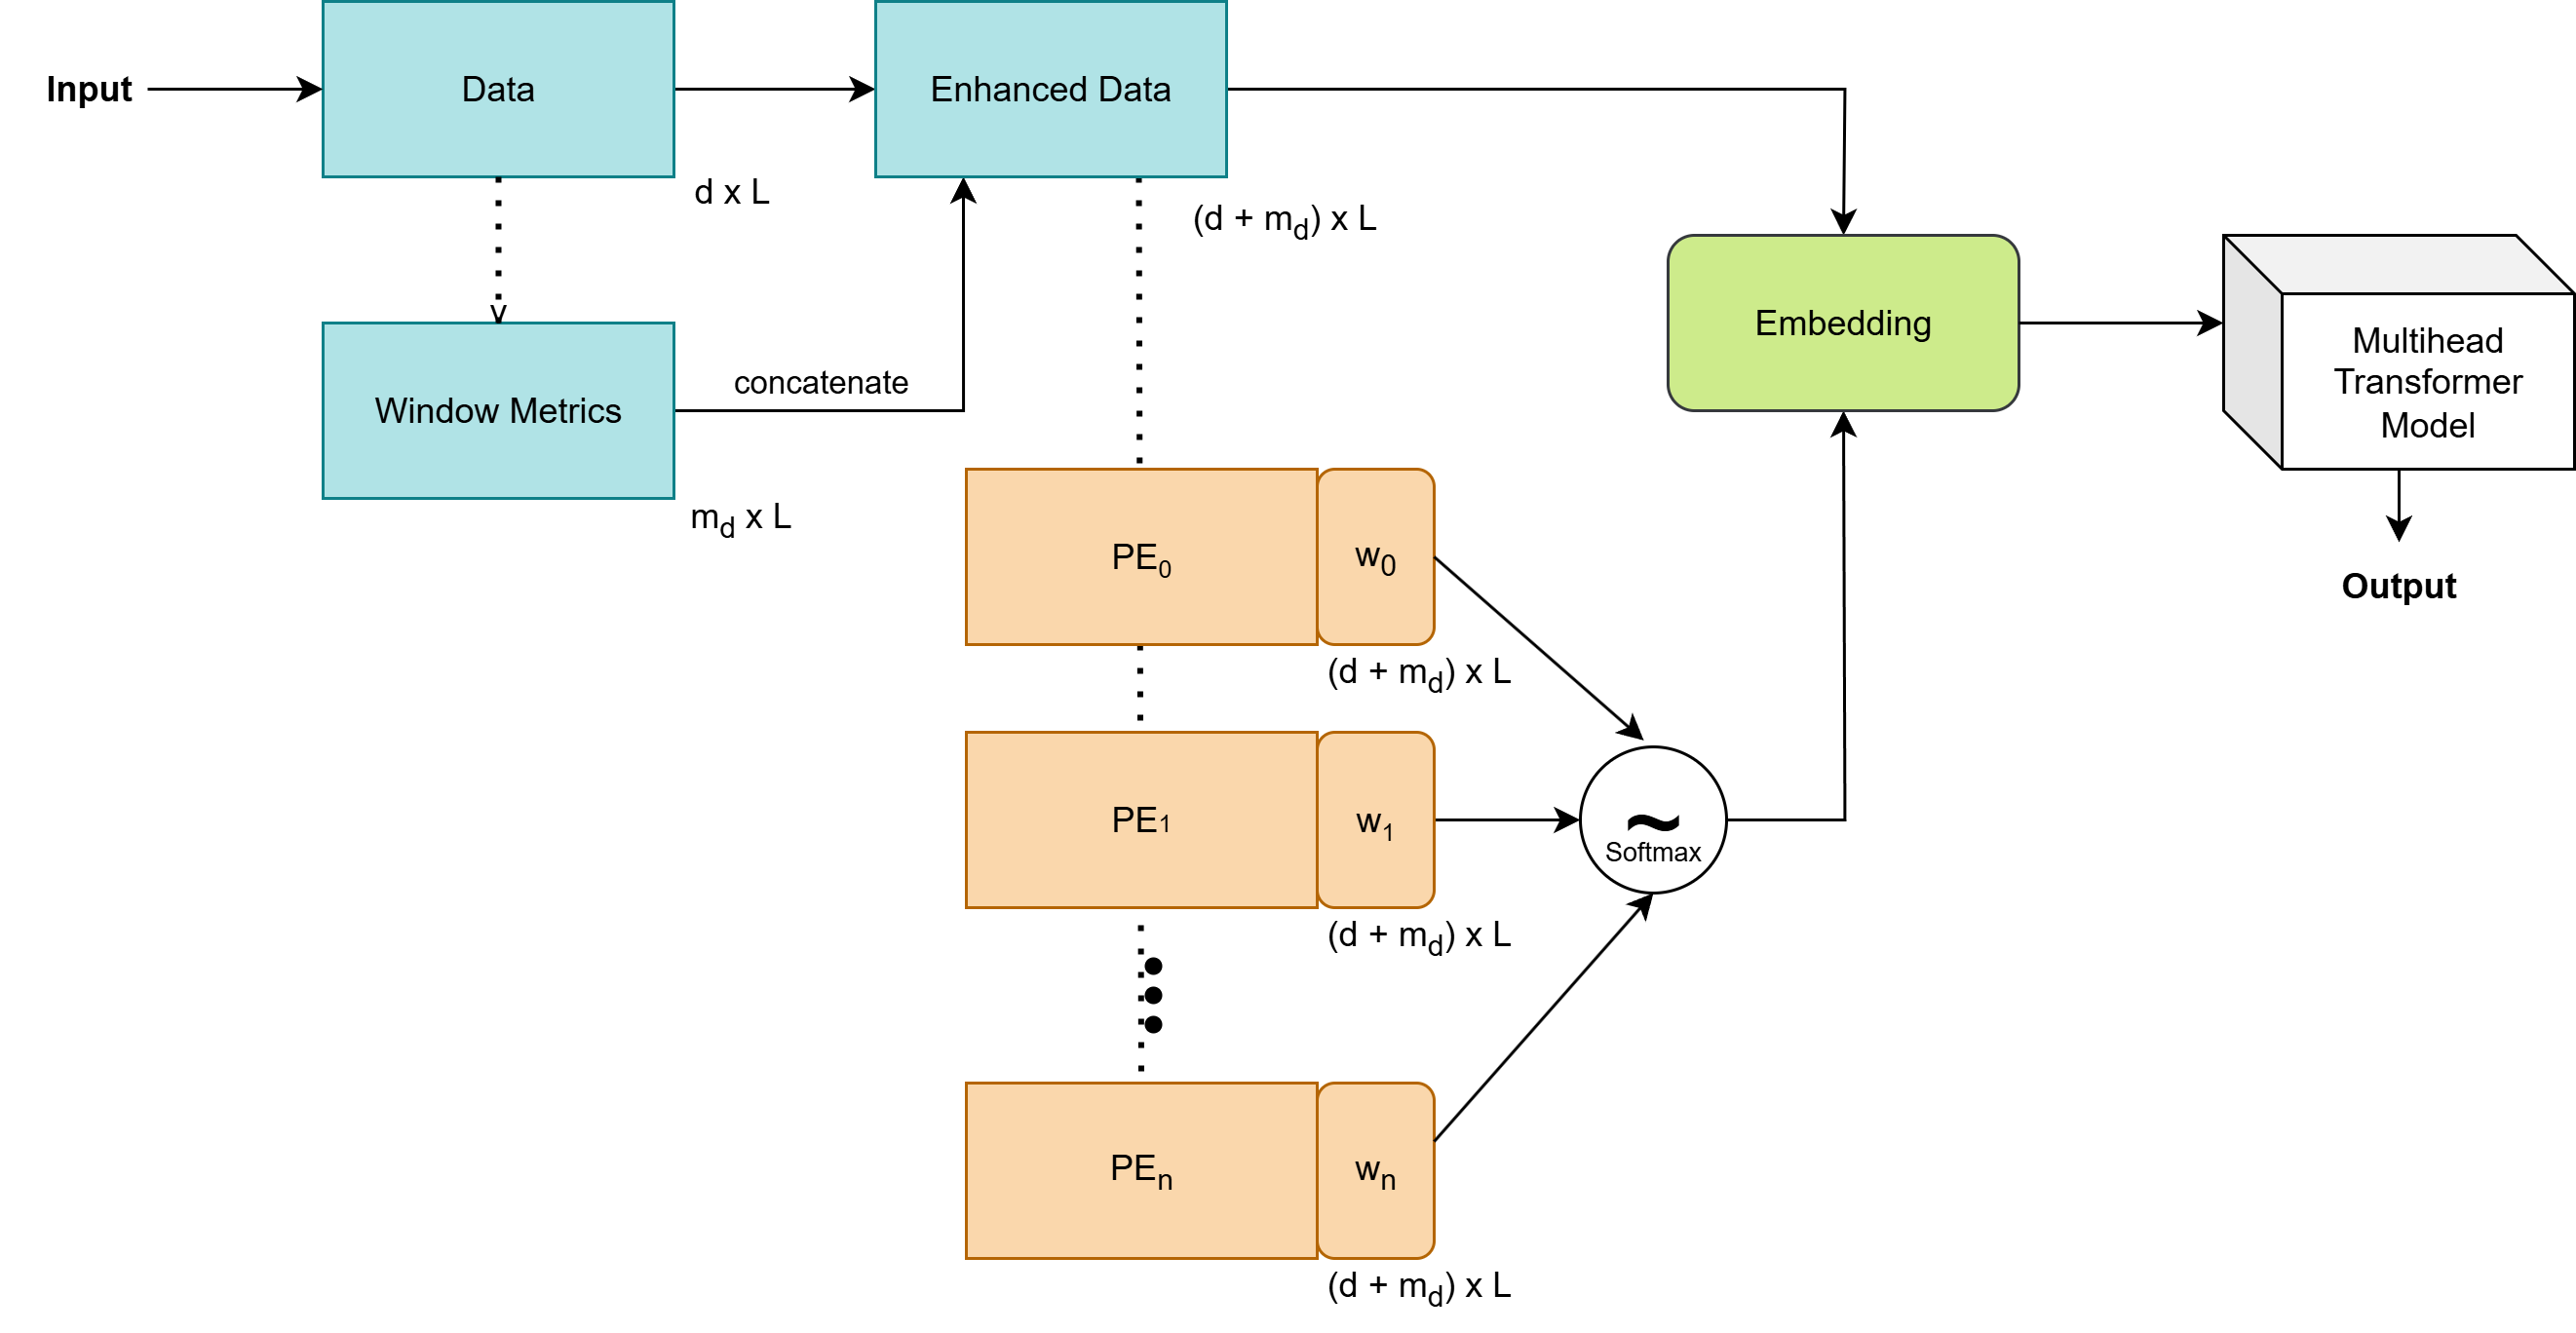
\includegraphics[scale=0.6]{img/enhancedhybrid.png}
	\caption{Propuesta: ponderación de métodos aditivos e información de ventana concatenada}
	\label{enhancedhybrid}
\end{figure}

Sea \(\mathbf{e}_0\in\mathbb{R}^d\) el embedding de partida, con la información adicional de ventana ya concatenada y \(\{\mathbf{pe}_k\}_{k=1}^K \subset \mathbb{R}^d\) los encodings que deseamos añadir. Para su ponderación, introducimos pesos aprendibles escalares \(w_k\in\mathbb{R}\), que normalizamos con Softmax:
\[
\alpha_k \;=\; \frac{\exp(w_k)}{\sum_{m=1}^{K}\exp(w_m)} \qquad (k=1,\dots,K).
\]
El embedding final es
\[
\mathbf{e}_{\mathrm{final}} \;=\; \mathbf{e}_0 \;+\; \sum_{k=1}^{K} \alpha_k\,\mathbf{pe}_k.
\]


De este modo, si \(\alpha_k \approx 0\) el encoding correspondiente queda suprimido. Y de forma algorítmica, quedaría de la siguiente forma:
\begin{itemize}
	\item Inicializar \(w_k\) con valores pequeños.
	\item Opcionalmente, usar clipping de gradientes o normalización/weight-normalization.
	\item Entrenar el modelo mientras se cumpla el número de épocas establecido o se llegue a una condición de parada.
\end{itemize}


Para evaluar la utilidad de esta estrategia, diseñaremos una serie de modelos de encoding que cumplan las propiedades descritas, organizados de forma incremental en complejidad. Es decir, cada nivel incorporará nuevas características, comenzando por propuestas basadas en la correspondencia de puntos mediante estadísticos en ventana, continuando con la adición de \textit{lags} y, finalmente, hibridando con modelos más elaborados del estado del arte revisados previamente, y empleando la técnica de ponderado. Esta construcción gradual nos permitirá realizar de forma directa un \textit{ablation study} que identifique la contribución específica de cada componente, y así ver en qué puntos la estrategia no es correcta para descartarla.\\

Por tanto, el camino seguido para evaluar las diferentes alternativas, quedaría resumida de la siguiente forma:

\begin{enumerate}
	\item \textbf{WinStat}. Se trata de un modelo que usará el método de ventana deslizante para adjuntar valores estadísticos a los datos de entrada. Adjuntará media, std, y extremos, por lo que aumenta en 4 dimensiones el embedding resultante.
	\item \textbf{WinStatLag}. Consiste en añadir, a la propuesta anterior, información acerca de un conjunto de lags anteriores, de manera que se calculan las diferencias y se agregan como una nueva característica a cada punto. De nuevo, se aumenta el tamaño del embedding, y depende del número de lags a incorporar.
	\item \textbf{WinStatFlex}. Consiste en combinar el método anterior de WinStatLag con una ponderación de los diferentes postional encoding de tipo aditivo vistos, a excepción de TPE, que se trata de un método híbrido. Para ello, se emplea la arquitectura vista en la figura \ref{enhancedhybrid}.
	\item \textbf{WinStatTPE}. Realiza la ponderación de los métodos aditivos con TPE, pero suprimiendo TAPE, cuya codificación podría incorporar demasiada redundancia.
	\item \textbf{WinStatSPE}. Prueba la utilidad de un modelo combinado con encodings aditivos, valores estadísticos y un mecanismo de atención modificado, concretamente SPE, que es el que mejores resultados mostró en \cite{irani2025positionalencodingtransformerbasedtime}. 
\end{enumerate}

En los siguientes puntos, examinaremos con detalle cada alternativa, atendiendo a la formulación propia de cada una de ellas.

\subsection{WinStat}

Este método introduce nueva información al conjunto de datos para cada posición de este, empleando para ello el cálculo de valores estadísticos que permitan ampliar el contexto de cada punto usando para ello una ventana W de tamaño definido. A diferencia de otros encodings vistos anteriormente, WinStat busca añadir información contextual de forma explícita en el conjunto de datos, a diferencia de los modelos aditivos, que de alguna manera añaden dicha información de manera implícita en los datos.

\subsubsection{Funcionamiento}

La justificación de realizar este procedimiento proviene de la falta de semántica que frecuentemente apreciamos a la hora de crear un embedding. Parte de este contexto viene dado por el entorno en el que se encuentra cada punto, ya que cuanto estudiamos el significado de la estacionalidad, vimos que existían períodos repetidos (con mayor o menor diferencia), y que es interesante saber en qué lugar de dicho período se encuentra un punto para corresponderlo con otro.\\

Con el uso de valores estadísticos extraídos de esta ventana, como la media, la desviación típica y los extremos máximo y mínimo, estamos añadiendo al conjunto de entrada explícitamente redundancia semántica acerca de la variabilidad local de los datos, de manera que la arquitectura encuentra dicha correspondencia entre puntos de manera más sencilla y explícita. Formalmente hablando, esto puede interpretarse como la introducción de un \textit{sesgo inductivo local}: el modelo recibe de forma explícita información que de otro modo tendría que inferir a partir de múltiples capas de atención.\\

En términos de complejidad, el coste adicional es $O(L \cdot w)$, siendo $w$ el tamaño de ventana, lo que resulta asumible para secuencias de larga duración.\\

Su idea, por tanto, es sencilla: se basa en la generación de un vector estadístico $s_t$ que recoge el contexto local en la ventana entorno al instante $t$. Al concatenar $s_t$ con el embedding original $x_t$, obtenemos $\tilde{x}_t$, un vector enriquecido que combina la representación de partida del token, junto a una codificación explícita de su contexto cercano dentro de W.

\subsubsection{Definición formal}

Supongamos $X = [x_1, x_2, \dots, x_L] \in \mathbb{R}^{L \times d}$ la secuencia de entrada, donde $L$ es la longitud de la secuencia y $d$ la dimensión del embedding original en cada posición. Definimos como ventana deslizante de tamaño $w \in \mathbb{N}$ centrada en cada posición $t$ de la siguiente forma:

\[
\mathcal{W}_t = \{ x_j \mid j \in [t - \lfloor w/2 \rfloor,\, t + \lfloor w/2 \rfloor] \cap [1, L] \}
\]

Donde tenemos especial cuidado para evitar problemas de desbordamiento en los extremos del embedding (primera y última posición). Para cada ventana $\mathcal{W}_t$, calculamos los estadísticos, considerando que las operaciones se aplican elemento a elemento sobre las $d$ dimensiones del embedding:

\begin{enumerate}
	\item \textit{Media}:
	\[
	\mu_t = \frac{1}{|\mathcal{W}_t|} \sum_{x \in \mathcal{W}_t} x
	\]
	\item \textit{Desviación estándar}:
	\[
	\sigma_t = \sqrt{ \frac{1}{|\mathcal{W}_t|} \sum_{x \in \mathcal{W}_t} (x - \mu_t)^2 }
	\]
	\item \textit{Mínimo}:
	\[
	m^{\min}_t = \min_{x \in \mathcal{W}_t} x
	\]
	\item \textit{Máximo}:
	\[
	m^{\max}_t = \max_{x \in \mathcal{W}_t} x
	\]
\end{enumerate}

Posteriormente, definimos el vector estadístico asociado a la posición $t$ como:

\[
s_t = [\,\mu_t,\, \sigma_t,\, m^{\min}_t,\, m^{\max}_t\,] \in \mathbb{R}^{4}
\]

Y, finalmente, el embedding enriquecido de la posición $t$ es:

\[
\tilde{x}_t = [\,x_t \, \| \, s_t\,] \in \mathbb{R}^{d+4}
\]

donde $\|$ denota la concatenación de vectores, en este caso, el del embedding de base y la nueva información contextual. El resultado global es la secuencia:

\[
\tilde{X} = [\,\tilde{x}_1, \tilde{x}_2, \dots, \tilde{x}_L\,] \in \mathbb{R}^{L \times (d+4)}
\]

que será la entrada de nuestro modelo de Transformer seleccionado.\\

De manera algorítmica, su implementación es bastante sencilla (ver pseudocódigo \ref{winstat}). Al usar herramientas del lenguaje de programación que permitan cálculo en paralelo, las operaciones son fácilmente vectorizables, reduciendo así el tiempo necesario para la creación del vector.

\begin{algorithm}[H]
	\begin{algorithmic}[1]
		\REQUIRE $X \in \mathbb{R}^{L \times d}$ (matriz de entrada), $w \in \mathbb{N}$ (tamaño de ventana)
		\ENSURE $\tilde{X} \in \mathbb{R}^{L \times (d+4)}$
		\FOR{$t = 1$ \TO $L$}
		\STATE $W_t \gets X[\max(1, t - \lfloor w/2 \rfloor) : \min(L, t + \lfloor w/2 \rfloor)]$
		\STATE $\mu_t \gets \text{mean}(W_t)$
		\STATE $\sigma_t \gets \text{std}(W_t)$
		\STATE $m^{\min}_t \gets \min(W_t)$
		\STATE $m^{\max}_t \gets \max(W_t)$
		\STATE $s_t \gets [\mu_t, \sigma_t, m^{\min}_t, m^{\max}_t]$
		\STATE $\tilde{x}_t \gets \text{concat}(x_t, s_t)$
		\STATE $\tilde{X}[t] \gets \tilde{x}_t$
		\ENDFOR
		\RETURN $\tilde{X}$
	\end{algorithmic}
	\caption{WinStat: funcionamiento algorítmico del método basado en ventana de estadísticos}
	\label{winstat}
\end{algorithm}

\subsection{WinStatLag}

Teniendo como base WinStat, este método puede verse como una ampliación. Conservando los valores estadísticos calculados para cada posición, este método introduce información proporcionada de lags anteriores, de manera que se evalúa la diferencia entre el valor actual y tantos valores anteriores como se desee. El objetivo sigue siendo el mismo: mejorar la semántica a través del contexto local.

\subsubsection{Funcionamiento}

El método WinStatLag amplía el enfoque de WinStat incorporando, además de la estadística local de cada posición, información explícita sobre la evolución temporal a través de diferencias con lags. Este mecanismo permite capturar no solo el estado local de la señal, sino también sus variaciones a corto, medio o largo plazo, según los retardos elegidos.\\

La inclusión de retardos añade una dimensión temporal explícita al embedding; mientras que los valores estadísticos resumen el vecindario inmediato mediante métricas agregadas (media, desviación estándar, mínimo y máximo), los lags añaden gradientes temporales que pueden ser críticos para identificar tendencias, oscilaciones o cambios abruptos. Esto es especialmente relevante en series temporales donde la dinámica entre instantes consecutivos  o separados a un tamaño de intervalo específico suponen información clave para comprender los siguientes valores.\\

Para controlar el funcionamiento, podemos definir la existencia de un parámetro $p = |\mathcal{L}|$, que se define implícitamente al especificar un vector $\mathcal{L}$ con las posiciones t-anteriores que se deben tener en cuenta, y controla cuántos retardos se incorporan y, por tanto, cuánta historia temporal se integra en la representación. Cada retardo añade $d$ dimensiones adicionales, lo que incrementa la capacidad descriptiva pero también el coste computacional. Por ello, la selección de retardos debe ser equilibrada y razonable, y no se deberían superar los 3 o 5 rezagos como máximo a menos que sea necesario.\\

Su concepto fusiona contexto estadístico local de las 4 métricas anteriores y el gradiente temporal obtenido al realizar las diferencias, convirtiéndolo en una herramienta teóricamente más robusta para tareas de predicción en dominios donde la forma de la señal y sus cambios temporales son igualmente importantes.

\subsubsection{Definición formal}

Comenzamos, de nuevo, por definir nuestro vector de entrada, $X = [x_1, x_2, \dots, x_L] \in \mathbb{R}^{L \times d}$, donde $L$ es la longitud y $d$ la dimensión del \textit{embedding} original. Sea $w \in \mathbb{N}$ el tamaño de ventana deslizante y $\mathcal{L} = \{\ell_1, \ell_2, \dots, \ell_p\}$ el conjunto de retardos considerados.\\

Para cada posición $t$, definimos la ventana deslizante:
\[
\mathcal{W}_t = \{ x_j \mid j \in [t - \lfloor w/2 \rfloor,\, t + \lfloor w/2 \rfloor] \cap [1, L] \}
\]

Calculamos los estadísticos locales como en WinStat, obteniendo nuestro vector estadístico:
\[
s_t = [\,\mu_t,\, \sigma_t,\, m^{\min}_t,\, m^{\max}_t\,] \in \mathbb{R}^4
\]

Y ahora, adicionalmente, para los retardos, definimos para cada $\ell_j \in \mathcal{L}$:
\[
\delta_t^{(\ell_j)} = | x_t - x_{t - \ell_j}|, \quad \text{si } t - \ell_j \geq 1
\]

El \textit{embedding} enriquecido de la posición $t$ está constituido por la concatenación de los valores estadísticos y las nuevas diferencias:
\[
\tilde{x}_t = [\,x_t \,\|\, s_t \,\|\, \delta_t^{(\ell_1)} \,\|\, \dots \,\|\, \delta_t^{(\ell_p)}\,] \in \mathbb{R}^{d + 4 + p}
\]
y por tanto, la secuencia enriquecida tendrá como dimensión 4 + número de rezagos p.
\[
\tilde{X} = [\,\tilde{x}_1, \tilde{x}_2, \dots, \tilde{x}_L\,] \in \mathbb{R}^{L \times (d+4+p )}
\]

A nivel algorítmico (ver pseudocódigo \ref{winstatlag}), buena parte del código será similar a WinStat, al cual tendrán que agregarse los valores de diferencia.

\begin{algorithm}[H]
	\begin{algorithmic}[1]
		\REQUIRE 
		$X \in \mathbb{R}^{L \times d}$ (matriz de entrada), 
		$w \in \mathbb{N}$ (tamaño de ventana),
		$\mathcal{L} = \{\ell_1, \ell_2, \dots, \ell_p\}$ (conjunto de retardos)
		\ENSURE 
		$\tilde{X} \in \mathbb{R}^{L \times (d + 4 + p)}$
		\FOR{$t = 1$ \TO $L$}
		\STATE $W_t \gets X[\max(1, t - \lfloor w/2 \rfloor) : \min(L, t + \lfloor w/2 \rfloor)]$
		\STATE $\mu_t \gets \text{mean}(W_t)$
		\STATE $\sigma_t \gets \text{std}(W_t)$
		\STATE $m^{\min}_t \gets \min(W_t)$
		\STATE $m^{\max}_t \gets \max(W_t)$
		\STATE $s_t \gets [\mu_t, \sigma_t, m^{\min}_t, m^{\max}_t]$
		\STATE Inicializar vector de diferencias: $\Delta_t \gets []$
		\FOR{cada $\ell_j \in \mathcal{L}$}
		\IF{$t - \ell_j \geq 1$}
		\STATE $\delta \gets |x_t - x_{t - \ell_j}|$
		\ENDIF
		\STATE Añadir $\delta$ a $\Delta_t$
		\ENDFOR
		\STATE $\tilde{x}_t \gets \text{concat}(x_t, s_t, \Delta_t)$
		\STATE $\tilde{X}[t] \gets \tilde{x}_t$
		\ENDFOR
		\RETURN $\tilde{X}$
	\end{algorithmic}
	\caption{Cálculo de WinStatLag: añadiendo la información de los lags diferenciados}
	\label{winstatlag}
\end{algorithm}

Al igual que en el caso de WinStat, usando las librerías adecuadas, como veremos más adelante, es posible paralelizar este código para reducir los tiempos de cálculo.

\subsection{WinStatFlex}

Hasta ahora, los métodos definidos han utilizado la estrategia de añadir contexto explícito al conjunto de datos de entrada, de manera que el tamaño del mismo crece. Ahora, es el momento de ver si estas adiciones permiten mejorar el rendimiento de los encodings aditivos, utilizando para ello, la estrategia anteriormente descrita en la figura \ref{enhancedhybrid}: usar, con la salida proprocionada por WinStatLag, diferentes encodings aditivos ponderados mediante el uso de pesos normalizados. A continuación, describiremos su funcionamiento en detalle.

\subsubsection{Funcionamiento}

Anteriormente, empleamos la información otorgada por los estadísticos calculados en la ventana, y un número definido de rezagos como método explícito para mejorar la semántica de los datos y facilitar así el proceso inductivo del modelo. Sin embargo, aunque por sí solo pudieran dar resultados positivos, es interesante verificar qué ocurre cuando combinamos esta solución con la codificación posicional aditiva, más tradicional.\\

Los métodos aditivos se caracterizan por añadir información absoluta de los datos, haciendo hincapié en crear una estructura que permita identificar el orden de los elementos de forma global, pero teniendo de cerca la eficiencia computacional como restricción a cumplir. Esta ha sido la estrategia seguida desde un primer comienzo por el Transformer original de Vaswani~\cite{vaswani2023attentionneed} y sus métodos de codificación sucesores vistos.\\

Todos ellos se basan en el uso de la información geométrica proporcionada por los senos y cosenos: el PE original, TAPE, TPE... pero también existía la codificación posicional aprendible, LPE, que nos permite codificar la información de la forma más cercana posible a la semántica de los datos. Dada la similaridad de todos estos métodos, y a la falta de criterio exacto en la que usar cada una de estas variantes, resulta interesante permitir que el modelo, de alguna manera, escoja a qué metodología darle preferencia, y es así como surge la idea formulada anteriormente de ponderar mediante pesos: el modelo podrá aprender dichos pesos, que son normalizados, para ver a qué codificación dar preferencia.\\

Dicho comportamiento nos permitirá adaptarnos a cada conjunto de entrada, y además, si estudiamos los valores finales de cada peso, ver cuáles son las necesidades del modelo: una mejora en la semántica, o por el contrario, una mayor necesidad de encoding absoluto. Recordando el funcionamiento de esta teoría de pesos, para este modelo concreto, necesitaremos 4 pesos: para PE, LPE, TAPE y para la propia información de valor, proporcionada por WinStat. De esta forma, logramos un enfoque flexible, el cual da nombre a esta estrategia.\\

En esta variante, mantendremos TPE al margen, al ser una estrategia parcialmente solapada con el funcionamiento del resto de modelos aditivos, para tratar de no hacer los modelos aditivos probados demasiado redundantes.

\subsubsection{Definición formal}

Como punto de partida, comenzaremos calculando el vector de entrada. Este proviene de la salida proporcionada del encoding previo realizado por WinStatLag, el cual recibe como entrada los datos originales, $X = [x_1, x_2, \dots, x_L] \in \mathbb{R}^{L \times d}$; $w \in \mathbb{N}$ el tamaño de ventana deslizante y $\mathcal{L} = \{\ell_1, \ell_2, \dots, \ell_p\}$ el conjunto de lags.\\


Calculamos los estadísticos locales como en WinStat, obteniendo nuestro vector estadístico:
\[
s_t = [\,\mu_t,\, \sigma_t,\, m^{\min}_t,\, m^{\max}_t\,] \in \mathbb{R}^4
\]

Y adicionalmente, los lags $\mathcal{L}$:
\[
\delta_t^{(\ell_j)} = | x_t - x_{t - \ell_j}|, \quad \text{si } t - \ell_j \geq 1
\]

Así obtenemos el anteriormente definido \textit{embedding} enriquecido, fruto de la concantenación de ambo vectores adicionales:
\[
\tilde{x}_t = [\,x_t \,\|\, s_t \,\|\, \delta_t^{(\ell_1)} \,\|\, \dots \,\|\, \delta_t^{(\ell_p)}\,] \in \mathbb{R}^{d + 4 + p}
\]

Posteriormente, antes de emplear estos datos como entrada del Transformer, se aplican los 3 encodings aditivos: PE, LPE y TAPE. Para cada instante pos:

\begin{enumerate}
\item PE: encoding sinusoidal
$$
PE_{(pos, 2i)} = \sin\left(\frac{pos}{10000^{\frac{2i}{d}}}\right)
$$

$$
PE_{(pos, 2i+1)} = \cos\left(\frac{pos}{10000^{\frac{2i}{d}}}\right)
$$

$$
X_{PE} = \tilde{x}_t + PE[pos]
$$
\item LPE:

$$
LPE_{(pos)} = W_{pos}, \quad W_{pos} \in \mathbb{R}^d
$$

$$
X_{LPE} = \tilde{x}_t + LPE[pos]
$$

\item TAPE:

\begin{equation}
	\centering
	\omega^{new}_k = k \cdot \frac{d_{model}}{L}
\end{equation}


\begin{equation}
	\begin{aligned}
		\text{TAPE}_{(pos,2i)} &= \sin\!\left( pos \cdot \omega^{new}_i \right) \\
		\text{TAPE}_{(pos,2i+1)} &= \cos\!\left( pos \cdot \omega^{new}_i \right)
	\end{aligned}
\end{equation}

$$
X_{TAPE} = \tilde{x}_t + TAPE[pos]
$$

\end{enumerate}

Los tensores obtenidos se ponderan mediante los pesos $w_0, w_1, w_2, w_3 \in [0,1] \subset \mathbb{R}$, los cuales se normalizan mediante la función Softmax para asegurar que la suma del vector de pesos $W = [w_0, w_1, w_2, w_3]$ sea siempre igual a 1:

\[
\tilde{w}_i = \frac{e^{w_i}}{\sum_{j=0}^3 e^{w_j}}, \quad i = 0,1,2,3,
\]
Donde $W = \tilde{W}$.
 Así, cada una de las codificaciones obtenidas, \(X_{PE}\), \(X_{LPE}\) y \(X_{TAPE}\), representa una secuencia enriquecida con diferentes características que podrá ponderarse y adecuarse a las necesidades del modelo automáticamente. 
\[
X_{\text{final}} = w_0 \tilde{X} + w_1 X_{PE} + w_2 X_{LPE} + w_3 X_{TAPE}, \quad \text{con} \quad \sum_{i=0}^3 w_i = 1.
\]

Algorítmicamente, se trata simplemente de implementar modularmente por separado cada componente, y aplicar en el paso de forward la normalización Softmax de los pesos aprendibles, los cuales intervienen en el aprendizaje por gradientes (ver pseudocódigo \ref{winstatflex}).

\begin{algorithm}[H]
	\begin{algorithmic}[1]
		\REQUIRE $X \in \mathbb{R}^{L \times d}$ (matriz de entrada), $w \in \mathbb{N}$ (tamaño de ventana), $\mathcal{L}$ (conjunto de retardos), $W = [w_0, w_1, w_2, w_3]$ (pesos)
		\ENSURE $X_{\text{final}} \in \mathbb{R}^{L \times (d + 4 + p)}$ (representación final)
		
		\STATE $\tilde{X} \gets \text{WinStatLag}(X, w, \mathcal{L})$ \COMMENT{Cálculo de embedding enriquecido}
		\STATE $X_{PE} \gets \text{PE}(\tilde{X})$ \COMMENT{Codificación sinusoidal}
		\STATE $X_{LPE} \gets \text{LPE}(\tilde{X})$ \COMMENT{Codificación aprendible}
		\STATE $X_{TAPE} \gets \text{TAPE}(\tilde{X})$ \COMMENT{Codificación TAPE}
		
		\STATE $\tilde{W} \gets \mathrm{Softmax}(W)$ \COMMENT{Normalización de pesos}
		
		\STATE $X_{\text{final}} \gets \tilde{w}_0 \cdot \tilde{X} + \tilde{w}_1 \cdot X_{PE} + \tilde{w}_2 \cdot X_{LPE} + \tilde{w}_3 \cdot X_{TAPE}$
		
		\RETURN $X_{\text{final}}$
	\end{algorithmic}
	\caption{Cálculo de WinStatFlex: proceso de adición de encodings}
	\label{winstatflex}
\end{algorithm}


De esta forma, obtenemos el comportamiento deseado, ponderable y flexible respecto al contexto de los datos.

\subsection{WinStatTPE}

En este cuarto método, se propone una leve modificación con respecto a la propuesta realizada por WinStatFlex: sustituir TAPE por TPE, reforzando así aún más la componente semántica de los datos, y nos permita analizar cómo se comporta esta codificación con el resto de modelos aditivos e información adicional concatenada.

\subsubsection{Funcionamiento}

En este caso, el funcionamiento empleado por esta metodología es bastante sencilla. Parte de la anterior codificación WinStatFlex, donde empleamos la información otorgada por los estadísticos calculados en la ventana, los rezagos y la ponderación de encodings aditivos, para retirar la utilización de TAPE y en su lugar añadir TPE.\\

Esta decisión ha sido tomada por la similaridad existente entre ambos métodos. Si bien la PE clásica también sería redundante en este contexto, pues coincide totalmente con la parte geométrica de TPE, en este caso sí que hemos preferido mantenerla, ya que así, realizando un breve estudio de los pesos, podremos ver si nuestra ponderación se beneficia de un mayor contexto semántico proporcionado por TPE, o si este entra en conflicto con la información ya explícitamente añadida y los PE absolutos son suficientes de por sí.\\

Manteniendo esta combinación ponderada, que sigue siendo de 4 elementos, seguimos logrando un enfoque flexible basado en los datos.


\subsubsection{Definición formal}

La definición de este método tiene como base la salida de WinStatLag. Por tanto, para no repetir dicha sección ya conocida, suponemos como entrada al conjunto de datos $\tilde{X}$, con un tensor perteneciente a $\mathbb{R}^{d + 4 + p}$, fruto de la concatenación de estadísticos, lags e información base proporcionada por $X  \in \mathbb{R}^4$.\\

Supuesta la entrada, se aplican sobre ella los 3 encodings escogidos: PE, LPE y T-PE. Para cada instante pos:

\begin{enumerate}
	\item PE
	$$
	PE_{(pos, 2i)} = \sin\left(\frac{pos}{10000^{\frac{2i}{d}}}\right)
	$$
	
	$$
	PE_{(pos, 2i+1)} = \cos\left(\frac{pos}{10000^{\frac{2i}{d}}}\right)
	$$
	
	$$
	X_{PE} = \tilde{x}_t + PE[pos]
	$$
	\item LPE:
	
	$$
	LPE_{(pos)} = W_{pos}, \quad W_{pos} \in \mathbb{R}^d
	$$
	
	$$
	X_{LPE} = \tilde{x}_t + LPE[pos]
	$$
	
	\item T-PE:
	Para la componente geométrica, se toma PE sinusoidal:
	\begin{equation}
		PE_{i, 2k} = \sin\left(\frac{i}{10000^{\frac{2k}{d}}}\right), \quad
		PE_{i, 2k+1} = \cos\left(\frac{i}{10000^{\frac{2k}{d}}}\right)
	\end{equation}
	
	Y para la semántica, la similitud, que se define como:
	
	$$S(i, j) = \exp\left( -\frac{\|x_i - x_j\|^2}{2\sigma^2} \right)$$
	
	Añadiéndose al encoding final de manera aditiva:
	
	$$T\text{-}PE(i) = PE(i) + S(i, j)$$
	
	$$
	X_{TPE} = \tilde{x}_t + T-PE[pos]
	$$
	
\end{enumerate}

Los tensores obtenidos se ponderan mediante los pesos $w_0, w_1, w_2, w_3 \in [0,1] \subset \mathbb{R}$, los cuales se normalizan mediante la función Softmax, y posteriormente, se realiza la suma ponderada de todos los elementos de entrada.

\[
\tilde{w}_i = \frac{e^{w_i}}{\sum_{j=0}^3 e^{w_j}}, \quad i = 0,1,2,3,
\]

\[
X_{\text{final}} = w_0 \tilde{X} + w_1 X_{PE} + w_2 X_{LPE} + w_3 X_{TPE}, \quad \text{con} \quad \sum_{i=0}^3 w_i = 1.
\]

A nivel de algoritmo, basta con tomar la base modular creada para WinStatFlex y añadir TPE en el lugar de TAPE (ver pseudocódigo \ref{winstattpe}).

\begin{algorithm}[H]
	\begin{algorithmic}[1]
		\REQUIRE $X \in \mathbb{R}^{L \times d}$ (matriz de entrada), $w \in \mathbb{N}$ (tamaño de ventana), $\mathcal{L}$ (conjunto de retardos), $W = [w_0, w_1, w_2, w_3]$ (pesos)
		\ENSURE $X_{\text{final}} \in \mathbb{R}^{L \times (d + 4 + p)}$ (representación final)
		
		\STATE $\tilde{X} \gets \text{WinStatLag}(X, w, \mathcal{L})$ \COMMENT{Cálculo de embedding enriquecido}
		\STATE $X_{PE} \gets \text{PE}(\tilde{X})$ \COMMENT{Codificación sinusoidal}
		\STATE $X_{LPE} \gets \text{LPE}(\tilde{X})$ \COMMENT{Codificación aprendible}
		\STATE $X_{TPE} \gets \text{TPE}(\tilde{X})$ \COMMENT{Codificación TPE}
		
		\STATE $\tilde{W} \gets \mathrm{Softmax}(W)$ \COMMENT{Normalización de pesos}
		
		\STATE $X_{\text{final}} \gets \tilde{w}_0 \cdot \tilde{X} + \tilde{w}_1 \cdot X_{PE} + \tilde{w}_2 \cdot X_{LPE} + \tilde{w}_3 \cdot X_{TPE}$
		
		\RETURN $X_{\text{final}}$
	\end{algorithmic}
	\caption{Cálculo de WinStatTPE: proceso de ponderado y adición de encodings}
	\label{winstattpe}
\end{algorithm}

Obteniendo de esta forma el embedding ponderado final, listo para ser introducido al Transformer para ser refinado y aprendido.


\subsection{PE combinado con SPE}


